\section{Maze Detector}
\label{sec:md}

    \marginpar{
        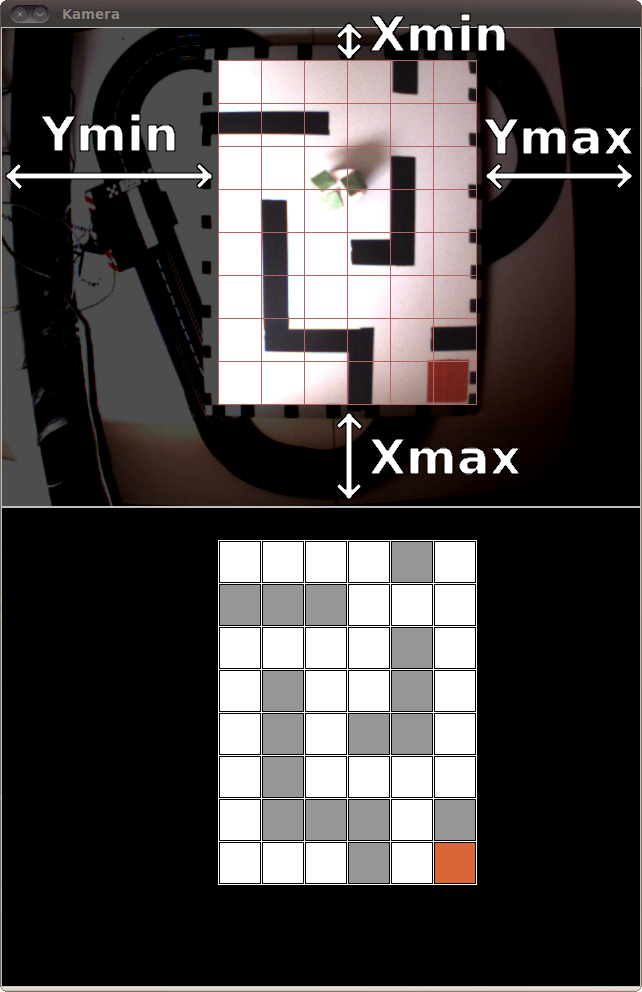
\includegraphics[width=4.5cm]{./img/MazeDetector_minmaxB.png}
        \captionof{figure}[Interface of Maze detector]{
        Interface of maze detector -- 
        The subframe can be adjusted to a specific region of the image
        using the $x_{min}$, $x_{max}$, $y_{min}$ and $y_{max}$ values.
        Only this region is considered by the detector.}
        \label{fig:md:interface}
    }

\subsection{Introduction}
\label{sec:md:intro}

The colored grid detector worked well to detect mean colors of the blocks, 
but it was too unstable in some circumstances, around the target for 
example. The mean color sometimes alternates quickly between two or 
three mean colors. To fix this, I built a subdetector that has two 
methods of detection. First, it detects the mean color and the closest 
mean color as for the Colored grid detector, but if the closest mean 
color is not close enough (distance bigger than max\_distance\_to\_color) 
then the detected color is the closest one between the wall color (by 
default black) and the ground color (by default white).

\subsection{Detection and drawing}
\label{sec:md:algo}
Here is the algorithm described in chronological order.

    \begin{enumerate}
        \item The detector enhances the colors given the saturation and 
            brightness values.
        \item It calculates the mean color of every block.
        \item It draws the mean color as a thick border inside blocks of 
            the upper image if print\_block\_color={\bf true}.
        \item It calculates the closest color from the mean block color.
        \item Set block color:
        \begin{enumerate}
            \item If the closest color is closest than a given threshold, 
                block color is set to the closest color value.
            \item Else, block color is set to closest color between 
                wall color and ground color.
        \end{enumerate}
        \item It draws the block selected color in the lower image 
        \item It adds blocks to the detected objects
        \begin{enumerate}
            \item $x$, $y$ (upper left corner)
            \item angle=0, size=color index (ground=0,wall=1)
        \end{enumerate}
        \item It draws the grid on the upper and lower image
        \item If in get\_block\_color mode, it draws the mean color of 
            the block in the lower image (get\_block\_x,get\_block\_y).
    \marginpar{
        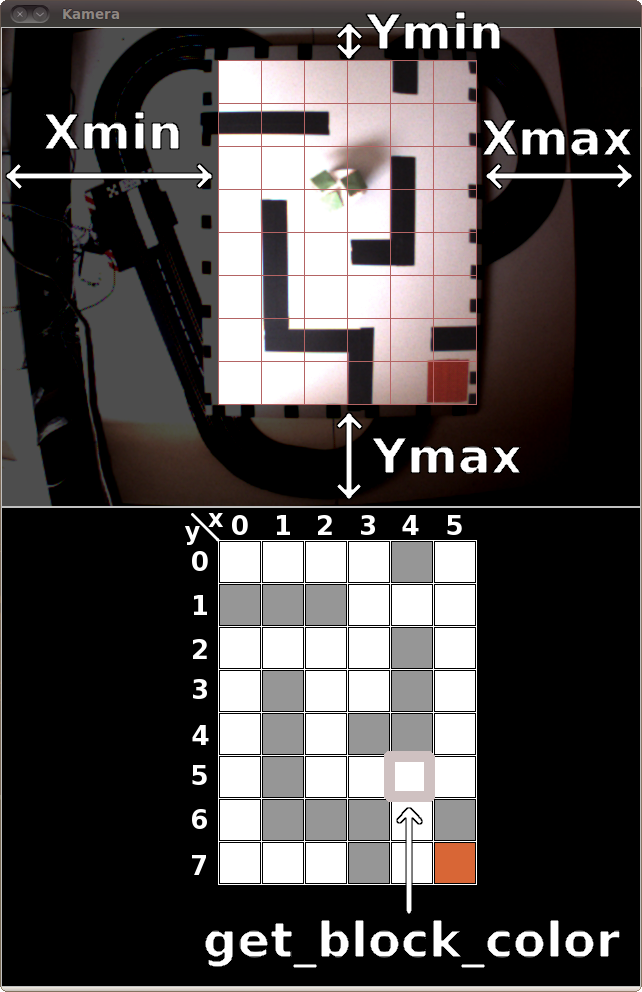
\includegraphics[width=4.5cm]{./img/MazeDetector_get_block_colorB.png}
        \captionof{figure}[Get\_object\_color mode]{%
        Get\_object\_color mode -- 
        This mode is really useful to get mean color value of 
        a given block. The mean color is also drawn as you can 
        see in the image at the end of the arrow.
        }
        \label{fig:md:getblockcolor}
    }
 
    \end{enumerate}

\subsection{Improvements}
\label{sec:md:improvements}

The same improvements of the colored grid detector apply to this one. 
See section \ref{sec:cgd:improvements} for more information.

\subsection{How to use}
\label{sec:md:howto}
    \begin{enumerate}
        \item Find colors that are easy to detect. Typically black and 
            white for the walls and the free space, and a basic color 
            like red for the target. An easy way to build it is with 
            red and black tape on a white board. Ground color is assigned
            to index 0 and wall color to index 1, the other colors given
            in the configuration file start their index at 2.
        \item You can build the maze before, but it is easier too build 
            it while the detector is on, so you can keep track of how 
            well it is detected.
        \item Once the camera is placed above the maze or the empty board, 
            set the $x_{min}$, $x_{max}$, $y_{min}$ and $y_{max}$
            values using the arrows to narrow 
            down the subframe around the maze
            (see figure \ref{fig:md:interface}). Be sure that the terminal 
            has the focus. Print on terminal the values by pressing
            the 'p' key. Write it down and 
            save the values in the configuration file.
        \item Use get\_block\_color mode to get the color values (RGB) 
            of the wall, the ground and the target (see 
            figure \ref{fig:md:getblockcolor}). Wall and ground 
            colors are black and white by default.
        \item You can adjust the brightness and saturation values to 
            get better results.
    \end{enumerate}

    \subsubsection{Parameters for configuration file}
    \label{sec:md:howto:params}
        \begin{description}
            \item[grid\_x] \hfill \\ int, Number of blocks in $x$.
            \item[grid\_y] \hfill \\ int,  Number of blocks in $y$. 
                (default = grid\_x)
            \item[x\_min] \hfill \\ int, Lower limit of the detection 
                frame on the image.
            \item[x\_max] \hfill \\ int, Upper limit of the detection 
                frame on the image.
            \item[y\_min] \hfill \\ int, Left limit of the detection frame 
                on the image
            \item[y\_max] \hfill \\ int, Right limit of the detection 
                frame on the image
            \item[print\_block\_color] \hfill \\ bool, Draws the mean 
                color of the block on the upper image
            \item[get\_block\_color] \hfill \\ bool, Enable the 
                get\_block\_color on start
            \item[get\_color\_x] \hfill \\ int,  Initial $x$ position of 
                get\_block\_color block
            \item[get\_color\_y] \hfill \\ int,  Initial $y$ position of 
                get\_block\_color block
            \item[saturation] \hfill \\ int,  Modify saturation of the 
                image
            \item[brightness] \hfill \\ int,  Modify brightness of the 
                image
            \item[colors] \hfill \\ int,int,int$|$int,int,int$|$..., given 
                colors to detect in RGB form
            \item[ground] \hfill \\ int,int,int, color of the ground 
                (default = 255,255,255)(white)
            \item[walls] \hfill \\ int,int,int, color of the walls 
                (default = 0,0,0)(black)
            \item[max\_distance\_to\_color] \hfill \\ int, maximal 
                distance to color before the block mean color
                is evaluated as ground or wall.
        \end{description}

    \subsubsection{Keys}
    \label{sec:md:howto:keys}

Press 'l', 'u', 'b', 's' or 'c' to enter a mode and 'e' to exit it. You can
then use the arrow and the 'p' key for the functionality of each mode.

    \begin{description} \itemindent=-15pt
        \item['l'] change minimum (left,up) bounds mode \\
            \begin{tabular}{ll}
                {\bf left } & $y_{min}$ -= 2 \\
                {\bf right} & $y_{min}$ += 2 \\
                {\bf up   } & $x_{min}$ -= 2 \\
                {\bf down } & $x_{min}$ += 2 \\
                {\bf 'p'  } & print $x_{min}$, $x_{max}$, $y_{min}$ and $y_{max}$
            \end{tabular}
        \item['u'] change maximum (right,down) bounds mode \\
            \begin{tabular}{ll}
                {\bf left } & $y_{max}$ -= 2 \\
                {\bf right} & $y_{max}$ += 2 \\
                {\bf up   } & $x_{max}$ -= 2 \\
                {\bf down } & $x_{max}$ += 2 \\
                {\bf 'p'  } & print $x_{min}$, $x_{max}$, $y_{min}$ and $y_{max}$ 
            \end{tabular}
        \item['b']  change brightness mode \\
            \begin{tabular}{ll} 
                {\bf left } & -5 to brightness \\
                {\bf down } & -5 to brightness \\
                {\bf right} & +5 to brightness \\
                {\bf up   } & +5 to brightness \\
                {\bf 'p'  } & print brightness value 
            \end{tabular}
        \item['s'] change saturation mode \\
            \begin{tabular}{ll}
                {\bf left } & -2 to saturation \\
                {\bf down } & -2 to saturation \\
                {\bf right} & +2 to saturation \\
                {\bf up   } & +2 to saturation \\
                {\bf 'p'  } & print saturation value \\
            \end{tabular}
        \item['c'] get\_block\_color mode \\
            \begin{tabular}{ll} 
                {\bf left } & move get\_block\_color block to the left  \\
                {\bf right} & move get\_block\_color block to the right \\
                {\bf down } & move get\_block\_color block down \\
                {\bf up   } & move get\_block\_color block up \\
                {\bf 'p'  } & print get\_block\_color block position and 
                              comparisons \\
                            & (distance) with mean color of 
                              the block and \\
                            & the given colors
            \end{tabular}
        \item['e'] exit current mode
    \end{description}
